\chapter{Behavioral-epidemic model}
\label{ch:epi_behav_model}
\section{Model description}

The newly developed model in this thesis, the Susceptible-Against-Heedless-Compliant-Infected-Recovered (SAHCIR) model, combines both epidemic and behavioral components, establishing an innovative approach to disease modeling. This model aims to bridge the epidemiological and social dynamics of an outbreak, integrating empirical observations to compare model outcomes with real-world data, as discussed in the article \cite{Proverbio_Tex_2024}. While some existing models combine these aspects, such as the one presented in \cite{Bulai2023}, they often rely on predefined assumptions about specific behaviors rather than direct empirical validation.

The SAHCIR  model incorporates a variety of behavioral stances towards safety measures, reflecting both proactive (pro-precaution) and non-compliant (anti-precaution) attitudes. The model also recognizes that, particularly during an epidemic's initial phase, a significant portion of the population may not follow safety measures—not out of skepticism, but due to a lack of awareness about the severity of the outbreak. Additionally, the model allows for government intervention through parameters that influence the spontaneous transition rate from the "Against" to the "Compliant" group, mirroring real-world public health policies aimed at promoting preventive behaviors. 

This model thus provides a more empirically grounded framework for understanding the interplay between public health dynamics and social behaviors, filling a gap in the literature by providing a model designed for direct confrontation with real-world data rather than solely hypothetical scenarios.

%ALTRI ASPETTI INSERITI WRT TO THE BASIC BEHAVIOR MODELthe waning of opinion, lack of interest, after the recovery \cite{Zuo2022,Kemp_2021} The fact that even in the I or R compartments population mantain an against or compliant behviors, not isolate this mechanism only in the S compartments, as done for example in \cite{Zuo2022}. 

The model is composed of two layers coupled together: a disease layer, describing the evolution of an epidemic, and a behaviour layer describing the transition among different behaviours during the epidemic development.
The behavioral layer has three possible compartments, as seen in Chapter \ref{sec:behavioral_model}: Heedles, Compliant, and Against.

\begin{itemize}
	\item[$H$:] Heedless, people careless of the risk associated with the infection;
	\item[$C$:] Compliant, people that want to avoid to becoming infected or infecting others
	\item[$A$:] Against, people who not see the epidemic as a risk and do not use protections or change their behaviour during the epidemic. 
\end{itemize}

In the model, behavioral dynamics are combined with a SIRS epidemic model to create seven distinct, mutually exclusive compartments that capture both disease states and behavioral responses. The Heedless behavior can only be adopted by individuals who are susceptible to infection. This reflects the assumption that when a new disease emerges, individuals lack sufficient information and, consequently, they behave "normally," without adopting safety measures.

As people transition through stages of infection and recovery, the model assumes they can gain awareness of the disease's risks and recognize the importance of infection prevention. Thus, after infection or recovery, it is considered unrealistic for them to remain Heedless. Non-heedless individuals are divided into two categories: Compliant, those who adopt behaviors to minimize further spread, and Against, who are aware but do not actively prevent transmission, possibly due to personal beliefs or low risk perception. 

Overall, we can recognize the following compartments:
\begin{itemize}
	\item[$S_H$:] Susceptible Heedless, the group where there is the majority of the population at the beginning of an epidemic. There is not much information about disease-associated risk and therefore the people in this compartment have no fear of becoming infected and do not modify their behaviors.
	\item[$S_C$:] Susceptible Compliant, the group composed of those who actively avoid becoming infected and use non-pharmaceutical interventions to limit the possibility of getting sick and of spreading the contagion.
	\item[$S_A$:] Susceptible Against, the people that do not comply with the recommendations provided by media or authority. They do not consider the threat represented by the disease and do not respect the safety rules or recommended behavior to avoid getting sick or infecting others. 
	\item[$I_C$:] Infected Compliant, people infected by the virus. This group receives infections coming from both $S_C$ and $S_H$ compartments, because it is considered that even those who have a "neutral" opinion about the risk associated with the infection change their minds when they become infected. The main behavior associated with this group is that safety measures such as quarantine are respected,which limits disease spread.
	\item[$I_A$:] Infected Against, compartment composed of the Against Susceptibles who became sick. They do not respect self-isolation, and spread the disease. 
	\item[$R_C$:] Recovered Compliant, compliant people that are healed from the infection and contribute to raising awareness about the risk associated with the disease. 
	\item[$R_A$:] Recovered Against, the part of the recovered formed by against healed from the infection. The most radicalized can be in this group. They are protected by immunity from a disease in which they do not believe of needing protection. 
\end{itemize}

The resulting system is described by the following system of differential equations: 
\begin{equation}
	\begin{cases}
		\dot{S_H} = - \psi k_1 S_H \cdot C - k_2 S_H \cdot A + \lambda_1 S_C + \lambda_2 S_A + \delta(1-\phi)R_C - \beta S_H \cdot I\\
		\dot{S_C} = \psi k_1 S_H \cdot C + \delta \phi R_C - \lambda_1 S_C - \beta \rho S_C \cdot I  \\
		\dot{S_A} = k_2 S_H \cdot A - \lambda_2 S_A - \beta S_A \cdot I + \delta R_A \\
		\dot{I_C} = \beta \rho S_C \cdot I + \beta S_H \cdot I + \psi k_3 I_A \cdot C - \lambda_3 I_C -  k_4 I_C \cdot A + \lambda_4 I_A - \gamma I_C\\
		 \dot{I_A} = \beta S_A \cdot I - \psi k_3 I_A \cdot C + \lambda_3 I_C + k_4 I_C \cdot A - \lambda_4 I_A - \gamma I_A\\
		 \dot{R_C} = \gamma I_C - k_6 R_C \cdot A + \lambda_6 R_A + \psi k_5 R_A \cdot C - \lambda_5 R_C - \delta R_C\\
		 \dot{R_A} = \gamma I_A + k_6 R_C \cdot A - \lambda_6 R_A - \psi k_5 R_A \cdot C + \lambda_5 R_C - \delta R_A\\
	\end{cases}
	\label{eq:epi_behavioural_eq}
\end{equation}

where
\begin{itemize}
	\item $A = S_A + I_A + R_A$ is the total fraction of Against individuals.
	\item $C = S_C + I_C + R_C$  is the total fraction of Compliant individuals.
	\item $I = \epsilon \cdot I_C + I_A$ is the fraction of infected people contributing to spreading the infection.
	\item $\psi$ is a parameter that represents an increased (if its value is larger than 1) incentive to transition to the Compliant group. It can be regarded as an intervention from an external mean-field global agent.
	\item $\phi$ is a normalized parameter, used to split the population while re-entering in the susceptible class in the Heedless or Compliant group. 
	\item $\rho$ is the protection factor of Compliant people that reduces their risk of becoming infected.
	\item $\beta$ is the infectivity rate associated with the disease.
	\item $\gamma$ is the recovery rate.
	\item $\delta$ is the rate at which immunity wanes (so that recovered people become susceptible again).
	\item $\epsilon$ specifies the fraction of compliant infected that participate in the infection process.
\end{itemize}

\begin{figure}
	\centering
	\includegraphics[height=0.8\linewidth]{1_corpo/figure/model_SAHCIR}
	\caption[Epidemic behavior model]{Epidemic behavioral model with compartments and fluxes.}
	\label{fig:epibehaviourmodelfigure}
\end{figure}

\section{Basic reproduction number calculation}
The first analysis that can be performed on the Behavioral Disease model is to compute its basic reproduction number. It is defined as the spectral radius of the next-generation matrix. Using the method outlined in \cite{van_den_Driessche_2017} and now briefly described, this quantity is calculated. To distinguish between this value, that is related to the whole model, and is thus influenced by both the social and epidemic layer, and the classic epidemic only Reproduction number, described in Section \ref{subsub:threshold}, we denote this quantity with the symbol $E_0$. It is the "Epidemic reproduction number". 
Consider $x = (x_1,x_2,...,x_n)^T$ a vector describing the number of individuals in each compartment. The compartments of infected are $m$, and the relation $m < n$ holds. 
Assume that the system has a disease free equilibrium (DFE), denoted as $x_0$: $x_0$ exist and is stable in the absence of the disease, so when the infected compartments have value equal to zero. Furthermore in the DFE the linearized equations for $x_1,x_2,...,x_m$ decouple from the other equations. Thanks to these assumptions it is possible to write the $m$ infected equations in the form:
\begin{equation}
\label{eq:next_gen1}
\frac{dx_i}{dt} = \mathcal{F}_i(x) - \mathcal{V}_i(x), \text{ for } i =1,2,...m
\end{equation}
The two terms appearing in equation \eqref{eq:next_gen1}, are $\mathcal{F}_i(x)$, the rate of appearance of new infected in the compartments $i$, and $ \mathcal{V}_i(x)$ the rate of other transitions between compartment $i$ and other infected compartments. It is assumed that each function is continously differentiable at least twice in each variable.

To describe the evolution of the system, the following matrix notations is adopted: 
\begin{itemize}
	\item $F = [\frac{d \mathcal{F}_i}{d x_j}(x_0)]$ with $1 \le i$, and $j \le m$.
	\item $V = [\frac{d \mathcal{V}_i}{d x_j}(x_0)]$ with $1 \le i$, and $j \le m$.	
\end{itemize} 
The matrices are both evaluated at the disease free equilibrium, where $x = x_0$, and have dimension $m \times m$, with $m$ being the number of infected compartments in the model. 
Using the defined matrices, according to \cite{van_den_Driessche_2002,van_den_Driessche_2017}, the Epidemic reproduction number $E_0$ for the model \eqref{eq:epi_behavioural_eq} at a disease free equilibrium, where all infected densities are zero, is given by:
\begin{equation}
E_0 = spec(FV^{-1})
\label{eq:R_0_eqn}
\end{equation}
The disease-free equilibrium is defined as a locally stable equilibrium of the system in which there is no disease.
The matrix $FV^{-1}$ is called next generation matrix, while $spec(M)$ is the spectral radius of a matrix M. To understand the entries of the matrix, consider perturbing a population at the DFE by introducing one infected individual in compartment $k$.

The $(j,k)$ entry of $V^{-1}$ is the average time that the individual spends in the compartment $j$. Instead, the $(i,j)$ entry of $F$ is the  rate at which infected in compartment $j$ produce new infections in $i$. In $F$ only individuals that become infected for the first time must be inserted, while other influxes in the $i$th compartment, must be considered in the $V$ matrix. Finally the entry $(i,k)$  in $FV^{-1}$ is the expected number of new infections in  $i$ produced by the infected individual originally introduced in $k$.

Considering the system dynamics presented in \eqref{eq:epi_behavioural_eq}, matrices $F$ and $V$ are

\begin{align}
F & = 
\begin{bmatrix}
	\beta \epsilon(\rho S_C + S_H) \quad & \beta(\rho S_C + S_H) \\
	\beta \epsilon S_A \quad& \beta S_A
\end{bmatrix} \\
V & = 
\begin{bmatrix}
	\lambda_3+k_4(S_A+I_A+R_A)+\gamma-\psi k_3 I_A \quad & k_4 I_C-\lambda_4-\psi k_3 (S_C+I_C + R_C)  \\
	\psi k_3 I_A - \lambda_3 - k_4 (S_A + I_A + R_A) \quad & \psi k_3 (S_C + I_C + R_C) - k_4 I_C + \lambda_4 + \gamma
\end{bmatrix}
\label{eq:next_gen_matrices}
\end{align}

Once the matrices composing the next-generation matrix are defined, the value of the epidemic reproduction number is calculated, resulting in:

\begin{equation}
	\begin{split}
		E_0 = &\frac{\beta}{\gamma} \cdot \frac{num}{den} \\
		num = &S_A(\gamma+\lambda_3+\epsilon \lambda_4)+ (S_H + \rho S_C)(\lambda_3+\epsilon \gamma+\epsilon \lambda_4) + ...\\
		& (S_A + S_H + \rho S_C)[(I_A-\epsilon IC)(k_4 - \psi k_3)+k_4(R_A+S_A)+\psi \epsilon k_3 (R_C+S_C)]\\
		den = &\lambda_3+\lambda_4+\gamma+k_4(A-I_C)+\psi k_3 (C-I_A)
	\end{split}
	\label{eq:epidemic_reproduction _number}
\end{equation}

To compute the value of $E_0$, the above expression must be evaluated at the DFE equilibria. Now it is determined how to compute them.

\subsection{DFE calculation}
To calculate the value of the DFE points of the system, consider the equations in system \eqref{eq:epi_behavioural_eq}, referring to them as $\dot{x_i} = f_i(x)$, with $i = 1,\dots,7$, corresponding to the seven different compartments that form the model. With $j$ is instead defined the compartments of infected in the model, and the condition that $j < 7$ holds.
Disease-free equilibria are solutions of the system in which no infection is present, so $x_j = 0$, and the differential expressions are equal to zero. Imposing these conditions, along with mass conservation, leads to the following system to solve:
\begin{align*}
	\begin{cases} 
		\dot{x_i} &= 0  \quad \quad   i = 1,...,7\\
		x_j &= 0	\quad \quad	 j \ge 1, j <7	\\
		\sum_{i = 1}^{7} x_i &= 1 \quad \quad i = 1,...,7 \\
	\end{cases}
	\label{eq:epi_behavioural_eq2}
\end{align*}

Solving the system of equations simbolically using Matlab, three disease free equilibria are found:

\begin{center}
\begin{tabular}{|>{\centering\arraybackslash}m{1.2cm}|c|c|c|c|}
	\hline
	\rule[0ex]{0pt}{2.5ex}  & $S_C$ & $S_H$ & $S_A$ & $E_0$ \\
	\hline
	\rule[0ex]{0pt}{2.5ex} type-A & 0  & 1 & 0  
	& $\frac{\beta}{\gamma} \frac{\lambda_3+\epsilon \gamma + \epsilon \lambda_4}{\lambda_3 + \lambda_4 + \gamma}$  \\
	\hline
	\rule[0ex]{0pt}{2.5ex} type-B & 0 & $\frac{\lambda_2}{k_2}$ & $1- \frac{\lambda_2}{k_2}$  
	& 	$\frac{\beta}{\gamma} \frac{\gamma +\lambda_3+\epsilon \lambda_4 + S_H \gamma(\epsilon-1)+k4 S_A}{\gamma+\lambda_3+ \lambda_4+ k_4 S_A}$  \\
	\hline
	\rule[0ex]{0pt}{2.5ex} type-C & $1 -\frac{\lambda_1}{k_1}$ & $\frac{\lambda_1}{k_1}$ & 0 
	& $ \frac{\beta}{\gamma} \frac{(S_H+ \rho S_C)(\lambda_3+\epsilon \gamma + \epsilon \lambda_4+ \psi \epsilon k_3 S_C)}{\lambda_3 + \lambda_4 + \gamma + \psi k_3 S_C}  $  \\
	\hline
\end{tabular}
\end{center}


For all equilibria, the corresponding values of $R_C$ and $R_A$ are equal to zero.

\section{Model simulations}
We now present an analysis of the model through a set of numerical simulations to observe how the system reacts and evolve with different sets of parameters is performed.
Performing an analysis similar to the one conducted for the behavior model alone is in fact too complex, as it involves numerous equations and parameters. Even though models similar to the one presented here have been analyzed in other works, such as \cite{Bulai2023}, those analyses often rely on strong assumptions. E.g. in \cite{Bulai2023} the hypothesis is the existence of different time scales between the epidemic and behavioral layers, enabling the simplification of the analysis. However, this assumption was deemed unreliable during the development of this model. Models intended to use empirical data, such as those related to epidemic evolution, typically rely on data collected on a daily basis. For this reason, it is assumed that the time scales of the epidemic and behavioral layers comparable. Although adopting the time-separation hypothesis might simplify the analysis, it would essentially yield the same results found in the behavior model alone. Thus, extensive simulations become crucial to enhance understanding of the model.

A first evaluation of $E_0$ is performed to assess its capability to provide indications about the stability of the equilibrium. As stated in \cite{van_den_Driessche_2002,van_den_Driessche_2017}, the DFE is locally asymptotically stable if $E_0 < 1$. Conversely, if $E_0 > 1$, a fully susceptible population, when perturbed by the introduction of infectious individuals, will progress toward an epidemic.

The same four cases of parameter configurations used in the previous chapter for the behavioral layer are employed here. For the epidemic layer, the value of $R_0$ is fixed at $3.2727$, based on the assumption of an average recovery period lasting $9$ days and a transmission rate similar to that estimated for diseases like COVID-19 at the early stages of its spread \cite{data_R0_covid}. An additional V case is introduced, in which the magnitudes of $\mathcal{B}_1$ and $\mathcal{B}_2$ are inverted relative to those in case IV.

To represent a wide range of scenarios, the epidemiological framework is kept constant, maintaining the same values for $\beta$, $\gamma$, and $\delta$ across all five cases. What varies is the intensity and relationship between the conversion numbers $\mathcal{B}_1$ and $\mathcal{B}_2$.

All computations are performed using the following fixed set of parameters:
\begin{align*}
\beta &= 0.40  &\gamma &= 0.35 & \delta &= 1/9 &  \epsilon &= 0.15 &\\
\epsilon &= 0.15 & \rho &= 0.65  &\psi &= 1 & \phi &= 0.5 &   \\	
\end{align*}
With these coefficient values, considering separately the epidemic and behavioral layers the basic epidemiological-only reproduction number of the SIRS model is:
 \begin{equation*}
 	R_0= \frac{\beta}{\gamma+\delta} = 3.2727 
 \end{equation*}
 
For the other behavioral coefficients it is assumed $k_3 = k_5 = k_1$, and $k_4 = k_6 = k_2$. Also $\lambda_3 = \lambda_5 = \lambda_1$, and  $\lambda_4 = \lambda_6 = \lambda_2$. 
The values of these coefficients change across the five cases.
\begin{center}
 \begin{tabular}{|c|c|c|c|c|}
 	\hline
 	& $B_1$ & $\lambda_1 \,[d^{-1}]$ & $B_2$ & $\lambda_2 \, [d^{-1}]$ \\
 	\hline
 	case I & 0.89 & 1/30 & 0.45 & 1/40 \\
 	\hline
 	case II & 8.5 & 1/40 & 8.5 & 1/20 \\
 	\hline
 	case III & 7 & 1/30 & 3 & 1/30 \\
 	\hline
 	case IV & 7 & 1/30 & 3 & 1/5 \\
 	\hline
 	case V & 3 & 1/30 & 7 & 1/2 \\
 	\hline
 \end{tabular}
\end{center}
The values of the variables $k_1$ and $k_2$ are derived using the expression $\mathcal{B}_i = k_i/\lambda_i$, where $i = 1, 2$.
The results of all simulations and the corresponding $E_0$ values are summarized in Table \ref{fig:valori-dfe-e-e0caso3}.

It is immediately noticeable how the value of $E_0$ changes and is influenced by both the behavioral parameters and the considered DFE.  The initial distribution of the population across compartments is chose by perturbing the computed DFE, through the insertion of some infected. The DFE type-$C$, where the population is divided between the Compliant and Heedless Susceptible compartments, is always locally asymptotically stable. In contrast, the type-$B$ equilibrium is always unstable, with $E_0>1$. A possible explanation for this observation lies in the effects of the parameters $\rho$ and $\epsilon$, which respectively reduce the likelihood of $S_C$ becoming infected and the ability of $I_C$ to infect others.
\begin{figure}[h]
	\centering
	\includegraphics[width=0.6\linewidth]{"1_corpo/figure/Valori DFE e E_0_caso_3"}
	\caption[$E_0$ simulation results]{The results of the simulations illustrate how $E_0$, the Epidemic Reproduction Number, varies across different possible scenarios.}
	\label{fig:valori-dfe-e-e0caso3}
\end{figure}
In the next paragraphs, the plots of the most relevant simulations for each of the five cases defined by these parameters are shown. In the simulations conducted using the Runge-Kutta second-order method, the number of infected individuals at time zero is slightly greater than zero: $I_{C0}= I_{A0} = 10/60e6$.

\subsection{I case: $\mathcal{B}_1, \mathcal{B}_2 <1$, $\mathcal{B}_1 >  \mathcal{B}_2$, and $\lambda_1 > \lambda_2$}
When calculating the Disease-Free Equilibrium (DFE), only one solution is found. It corresponds to the state $S_{C_0} = 0$, $S_{A_0} = 0$, and $S_{H_0} = 1$. In this equilibrium, the value of $E_0 = 1.142$, is greater than one. Therefore, as stated in the theorem presented in \cite{van_den_Driessche_2017}, the DFE is unstable, and a disease can evolve into an epidemic from this initial condition.

Observing the behavior layer, since both Conversion numbers $\mathcal{B}_1$ and $\mathcal{B}_2$ are less than one, the majority of the population remains in the Heedless compartment in this scenario. This facilitates disease propagation because only a small portion of individuals are in the Susceptible-Compliant ($S_C$) category, reducing their likelihood of infection, governed by $\rho \beta$ with $\rho < 1$. Meanwhile, $S_A$ and $S_H$ share the same probability of contracting the disease, $\beta$.

In the left panel of Figure \ref{fig:sim_B1_B2_less_equal}, it is evident that the dynamics are dominated by the Heedless compartment. Furthermore, an infection peak is observed, and the final equilibrium reached by the system is not disease-free: a relatively small portion of the population remains infected.

\begin{figure}[h]
	\centering
	\subfloat[][Case I: Both $\mathcal{B}_1$ and $\mathcal{B}_2$ are less than one. None of the possible behaviors become dominant.]
	{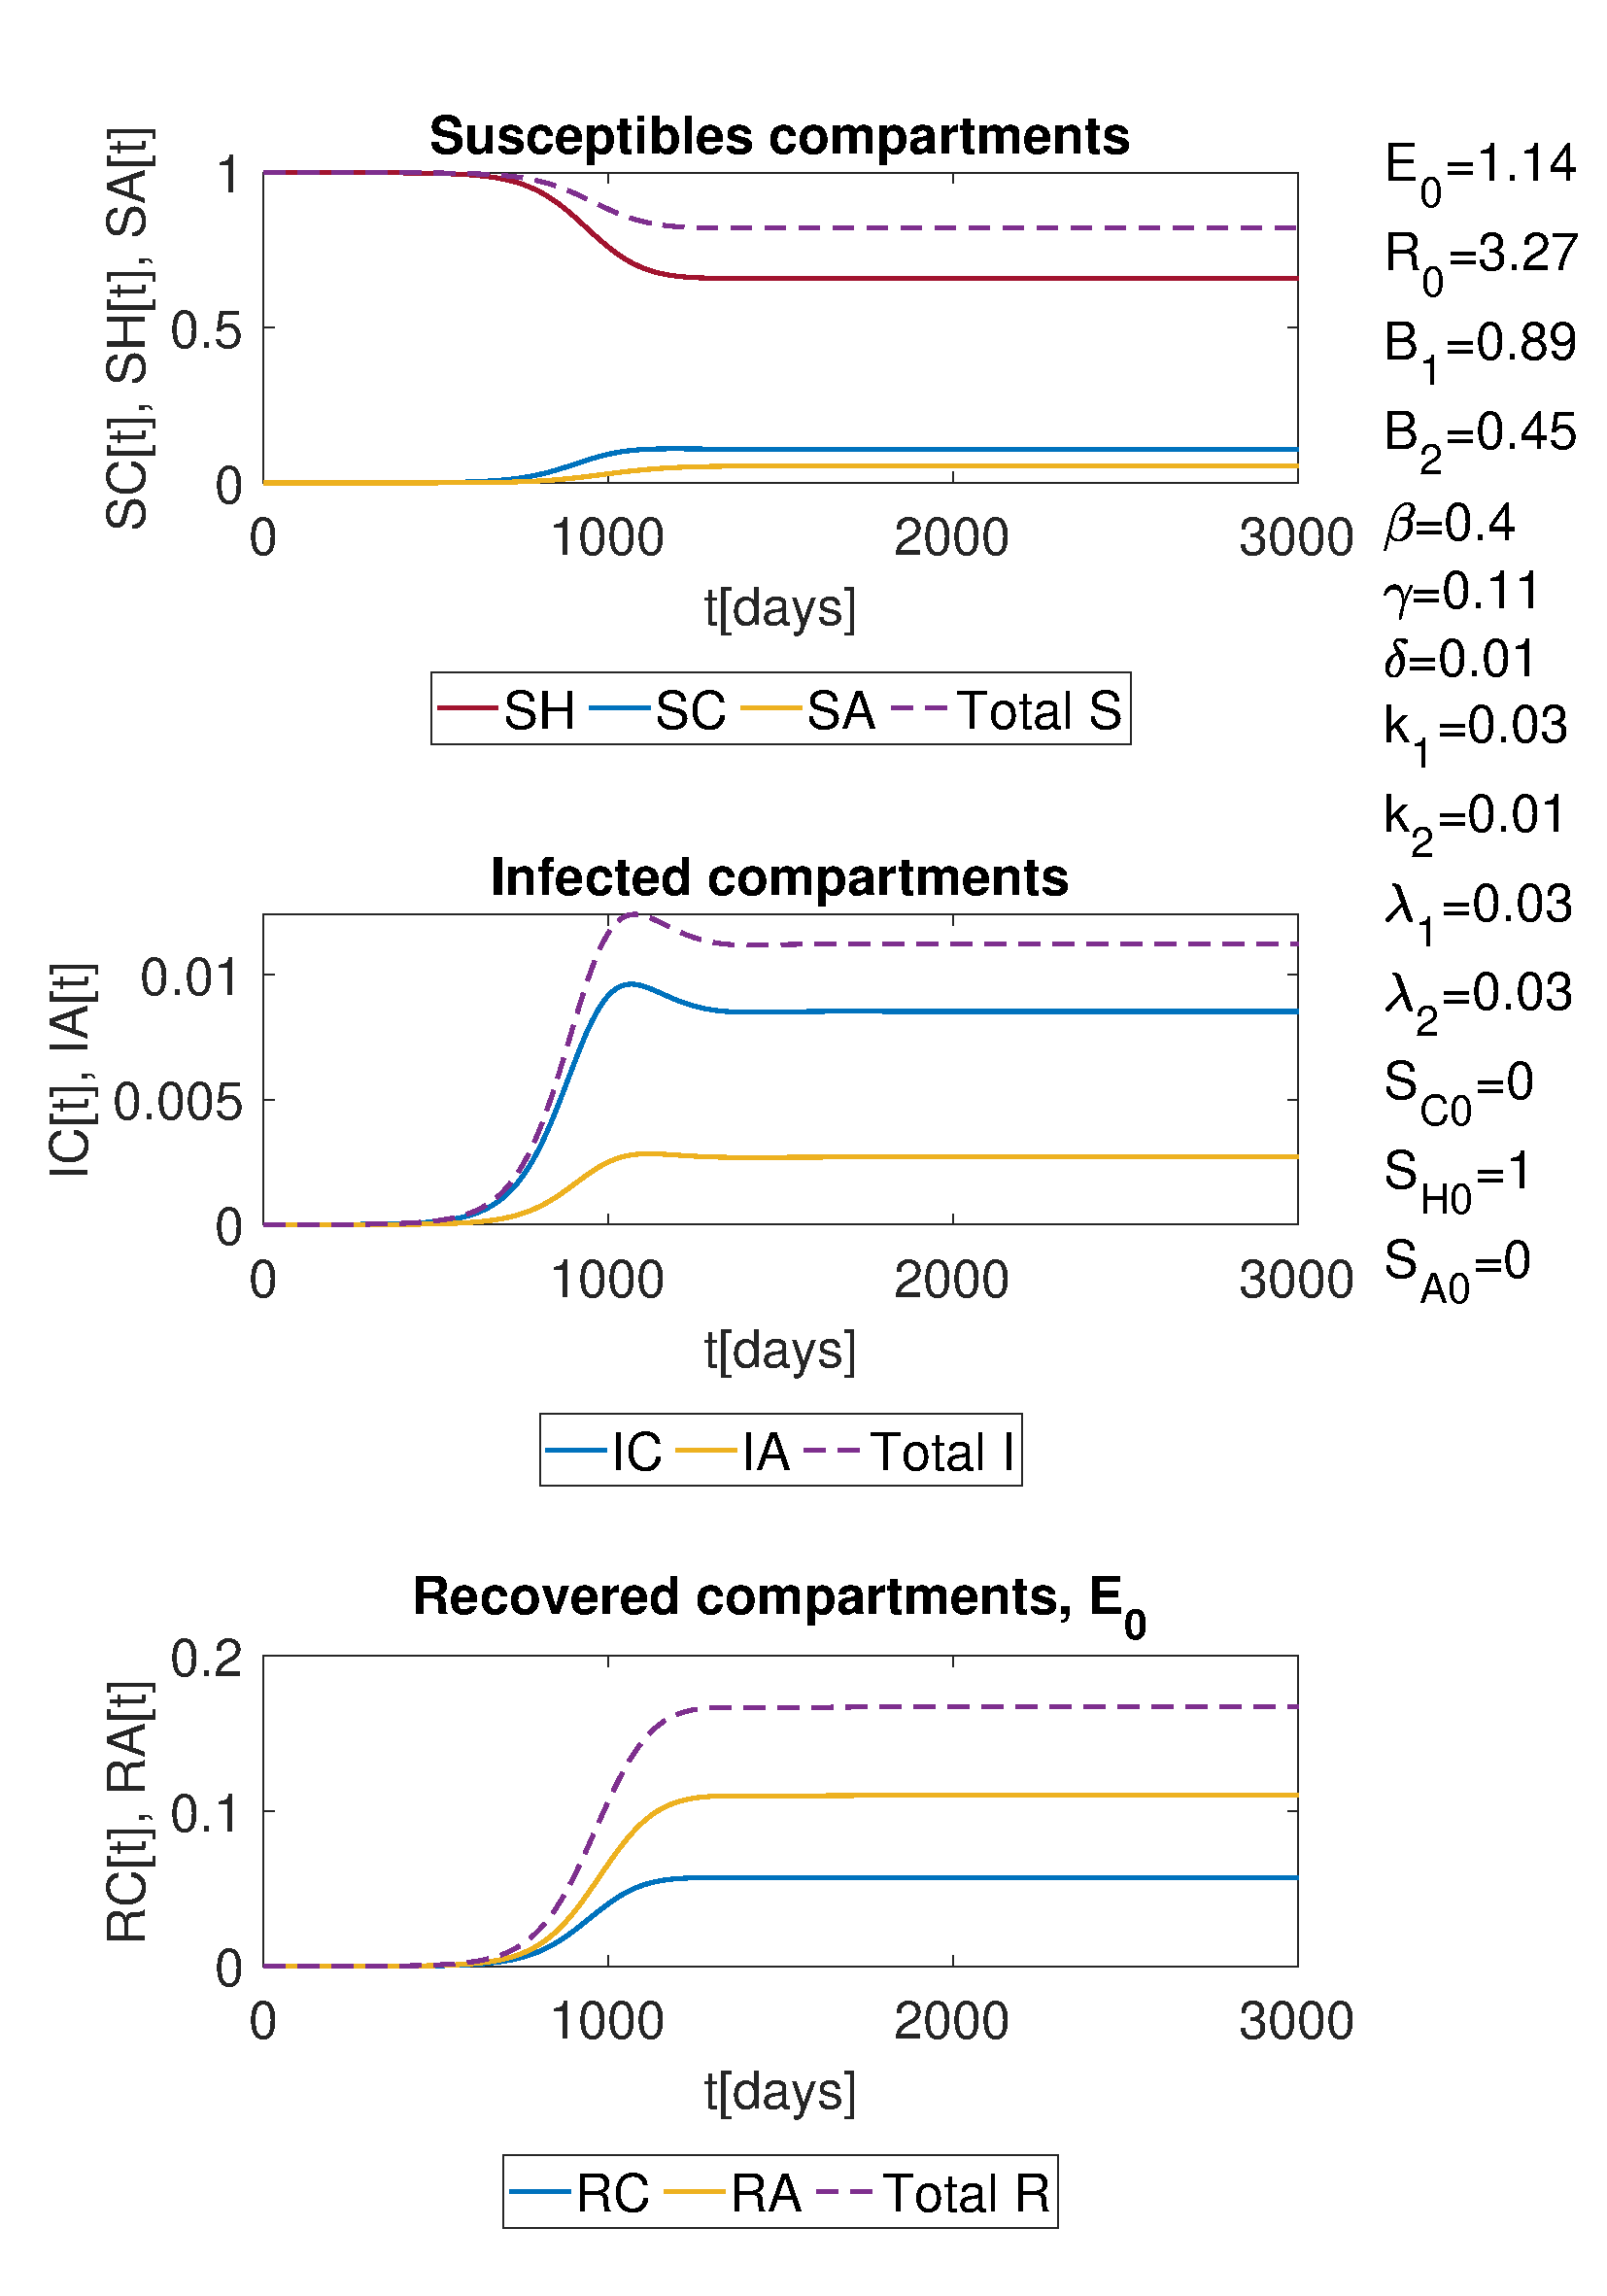
\includegraphics[width=0.48\linewidth]{1_corpo/figure/behav_epi_sim/E_0_model_1epi_behav_sim_B1_B2_less_1}} \quad
	\subfloat[][Case II: $\mathcal{B}_1$ is equal to $\mathcal{B}_2$. Starting from a type-C DFE, we have an $E_0$ that confirms the local asymptotic stability of the equilibrium. No epidemic develops in the system, as shown in the simulation.]
	{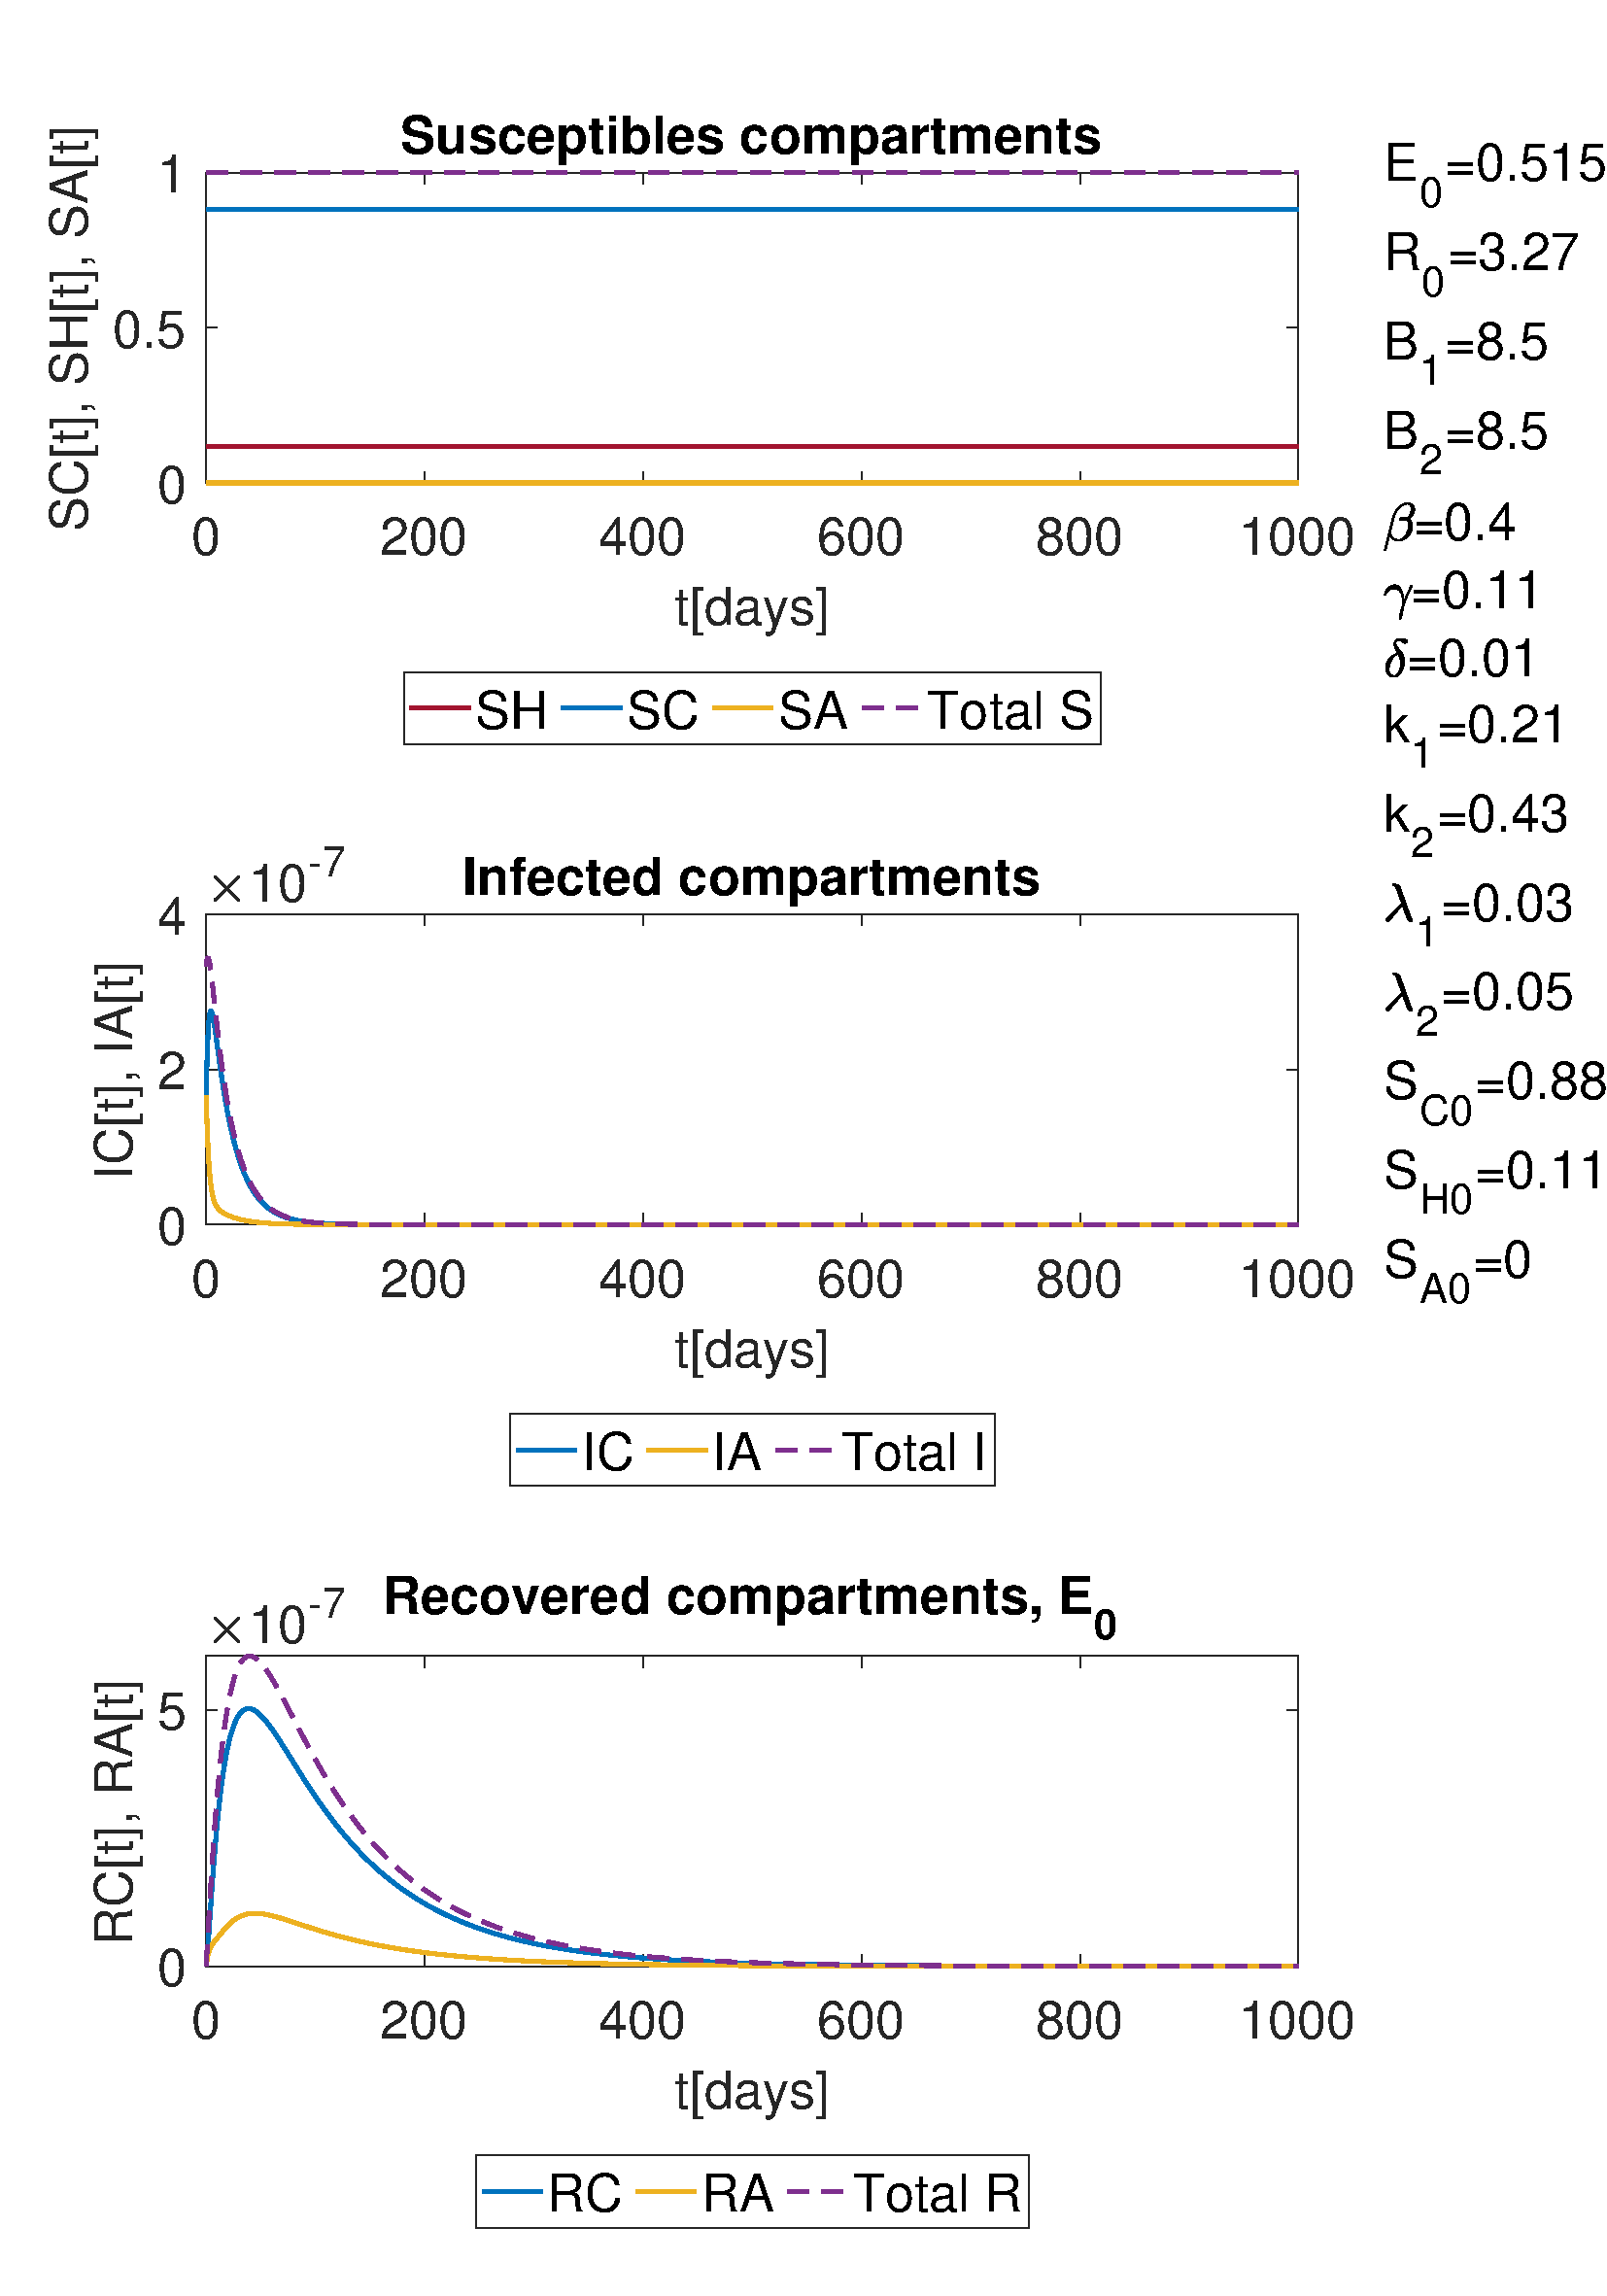
\includegraphics[width=0.48\linewidth]{1_corpo/figure/behav_epi_sim/E_0_model_2epi_behav_sim_B1_B2_equal}} \\
	\caption[Full model simulation figure first]{Cases I and II of the simulations performed. In the left panel, there is an epidemic outbreak leading to an endemic equilibrium, while in the right panel, the disease dies out, and the population remains in the Susceptible compartment at equilibrium.}
	\label{fig:sim_B1_B2_less_equal}
\end{figure}

\subsection{II case: $\mathcal{B}_1, \mathcal{B}_2 >1$, $\mathcal{B}_1 =  \mathcal{B}_2$, and $\lambda_1 < \lambda_2$}
If both behavioral layers have the same behavior conversion number,$\mathcal{B}_1 = \mathcal{B}_2$, as shown in the right panel of Figure \ref{fig:sim_B1_B2_less_equal}, the epidemic evolution is heavily influenced by the initial compartment values. This property holds even when the balance of the Behavior reproduction number is achieved with different coefficient values. Recall that $k_1$ and $k_2$ determine which behavior becomes dominant, while $\lambda_1$ and $\lambda_2$ impact the persistence of a certain behavior. In this case, the Compliant course of action is more dominant and slightly less persistent. However, the initial conditions plays a critical role in shaping the model evolution. When perturbing the type-C equilibrium, where the majority of the population is in the Compliant compartments, the population remains largely Compliant. Even when some infected individuals are introduced to perturb the disease-free state, the infection is rapidly suppressed. The equilibrium DFE, with a value of $E_0 = 0.515$, is locally asymptotically stable.


\subsection{III case: $\mathcal{B}_1, \mathcal{B}_2 >1$, $\mathcal{B}_1 <  \mathcal{B}_2$, and $\lambda_1 = \lambda_2$}
Figure \ref{fig:sim_B1_mag_B2}, explores the impact of compliance with rules and the adoption of self-precautions on the diffusion of an epidemic. Starting from the disease-free equilibrium type-$A$, where $S_{C0} = 1$ and all other compartments are equal to zero, the introduction of infected individuals triggers the spread of an infection. The value of $E_0 = 1.11$ indicates that the DFE is in fact unstable.

Although the disease can spread in a fully susceptible population, the protection provided by compliant behavior significantly reduces its spread. With $\mathcal{B}_1$ larger than $\mathcal{B}_2$, compliant behavior quickly spreads throughout the population and persists longer than the infection duration. As a result, the majority of the population transitions to the $S_C$ compartment, while $S_A$ tends toward zero. The epidemic fades after reaching a small peak and infecting only a minor fraction of the population.

\begin{figure}[h]
	\centering
	\subfloat[][\emph{III case.}]
	{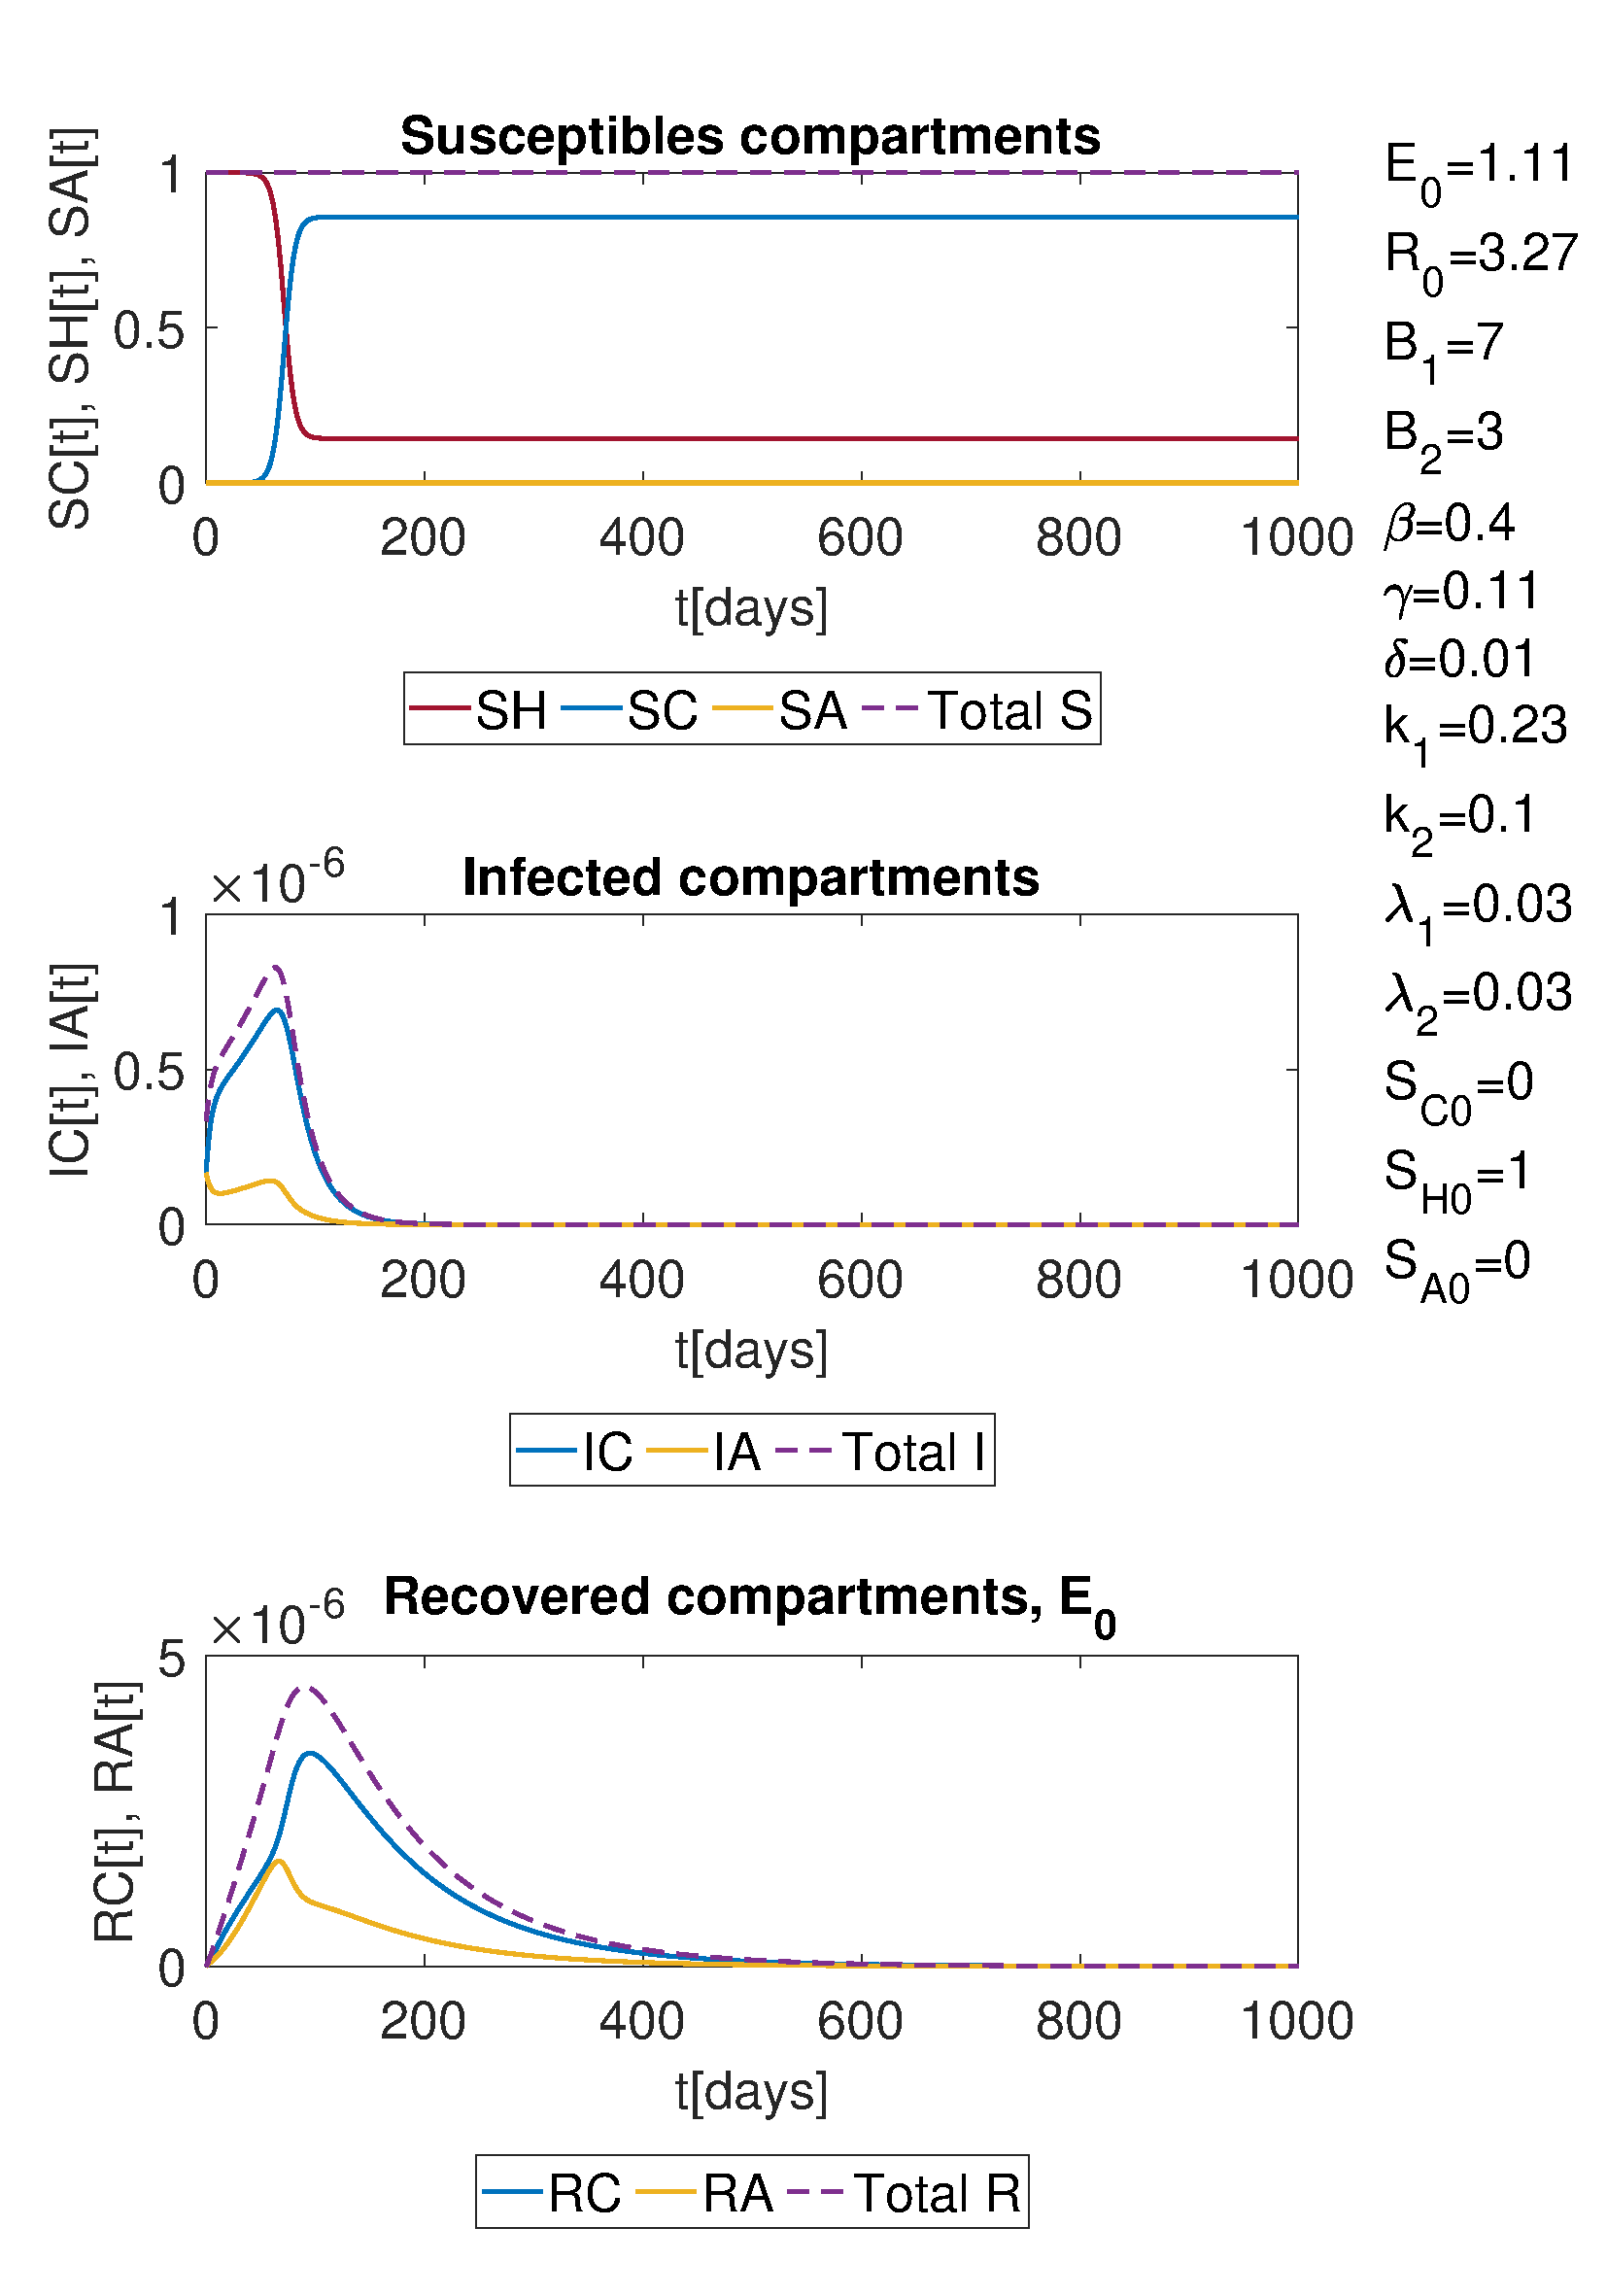
\includegraphics[width=0.48\linewidth]{1_corpo/figure/behav_epi_sim/E_0_model_1epi_behav_sim_B1_mag_B2}} \quad
	\subfloat[][\emph{ IV case.}]
	{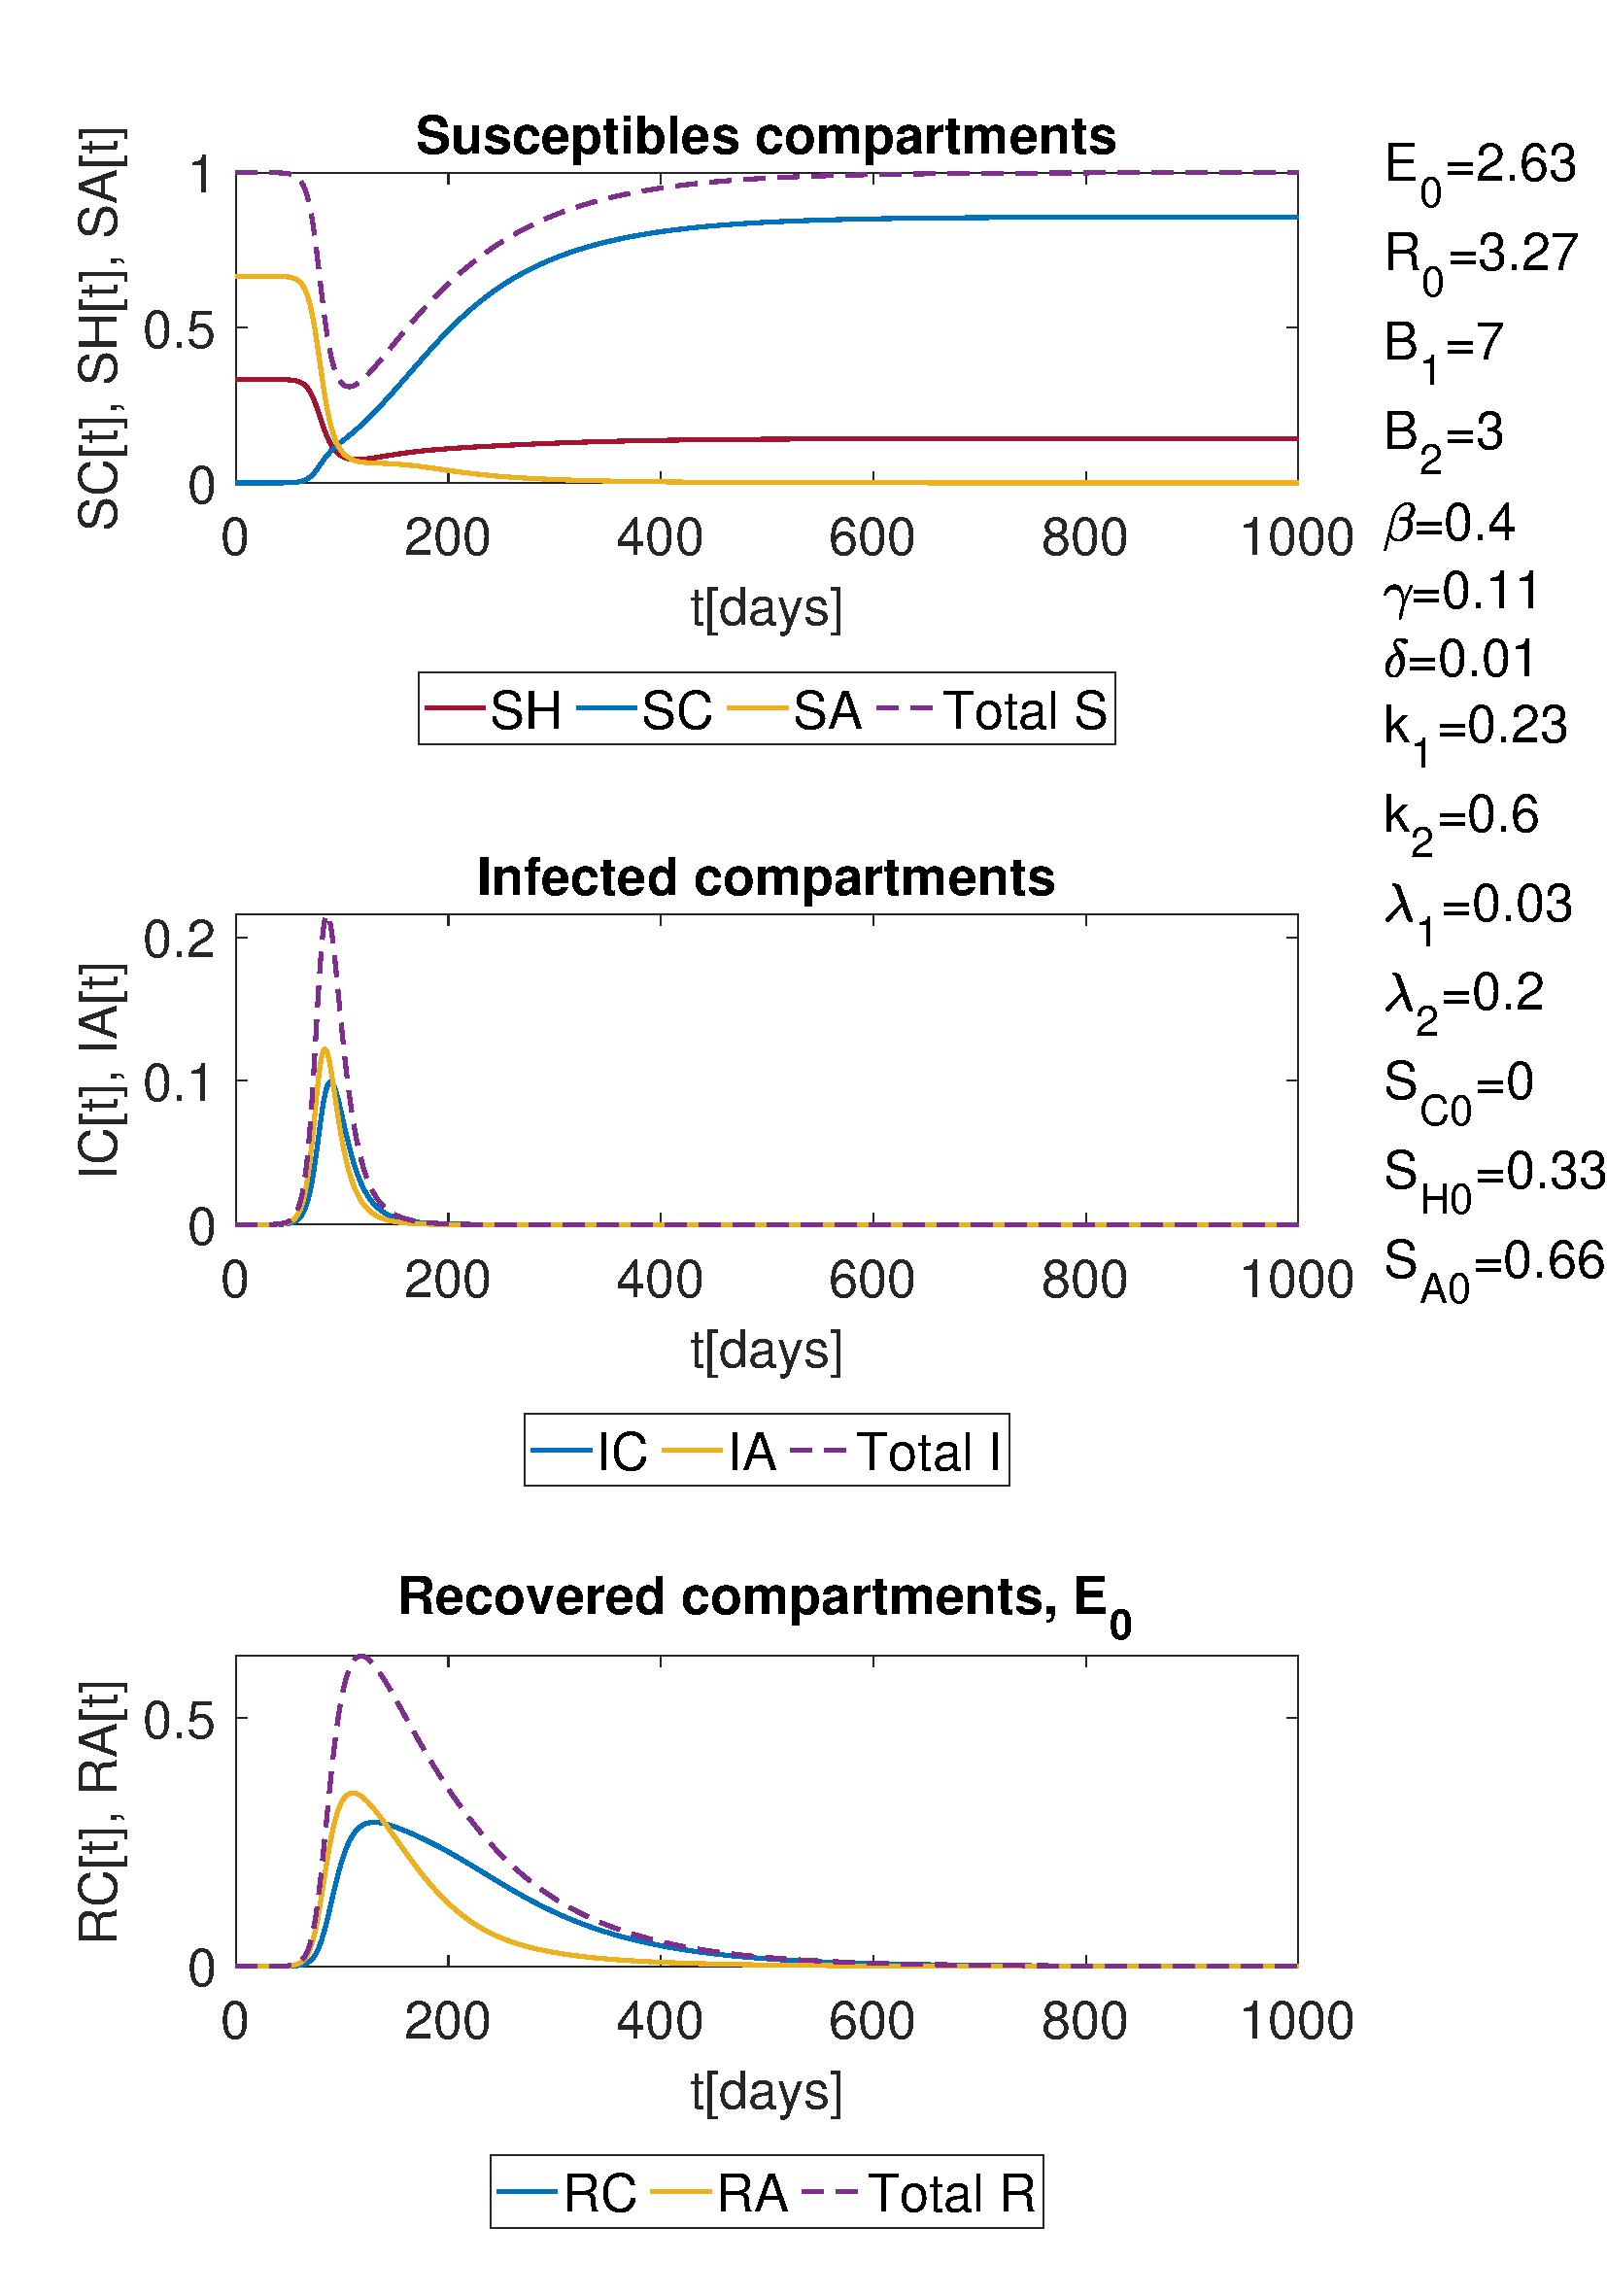
\includegraphics[width=0.48\linewidth]{1_corpo/figure/behav_epi_sim/E_0_model_2epi_behav_sim_B1_mag_B2_lambda2_mag}} \\
	\caption[Full model simulation figure second]{III and IV cases.}
	\label{fig:sim_B1_mag_B2}
\end{figure}


\subsection{IV case:  $\mathcal{B}_1, \mathcal{B}_2 >1$ and $\mathcal{B}_1 >  \mathcal{B}_2$, and $\lambda_1 < \lambda_2$}
The fourth case highlights and describes the negative effects of non-compliant behavior. Even though $\mathcal{B}_2 <\mathcal{B}_1$, the condition $k_2 \gg k_1$ allows the Against behavior to initially spread more rapidly. As observed previously with the behavior model alone in Section \ref{par:behav_4_case}, this dynamic results in significant early non-compliance. The simulation begins close to the DFE corresponding to type-B, where the majority of the population is in $S_A$. These initial conditions lead to a higher epidemic reproduction number, with $E_0 = 2.63$. Consequently, the number of infected individuals reaches a much higher peak compared to the third case.
However, as the simulation progresses, the Compliant group gradually gains prevalence due to $\mathcal{B}_1 >\mathcal{B}_2$. The population tends to shift toward compliance, and after the peak, the disease diminishes toward zero.

\subsection{V case:  $\mathcal{B}_1, \mathcal{B}_2 >1$ and $\mathcal{B}_1 <  \mathcal{B}_2$}
The final case represents the worst scenario for epidemic spread. The majority of the population adopts the Against behavior, which prevents the epidemic from being mitigated by NPIs or self-isolation. These measures are only adopted by an increasingly smaller portion of individuals. As a result, the epidemic trajectory closely resembles that of an SIRS-only model. With $E_0 = 3.17$, the highest value among all the cases presented, the infection peak is large, and the disease does not disappear. Instead, the system reaches an endemic equilibrium.

\begin{figure}[h]
	\centering
	{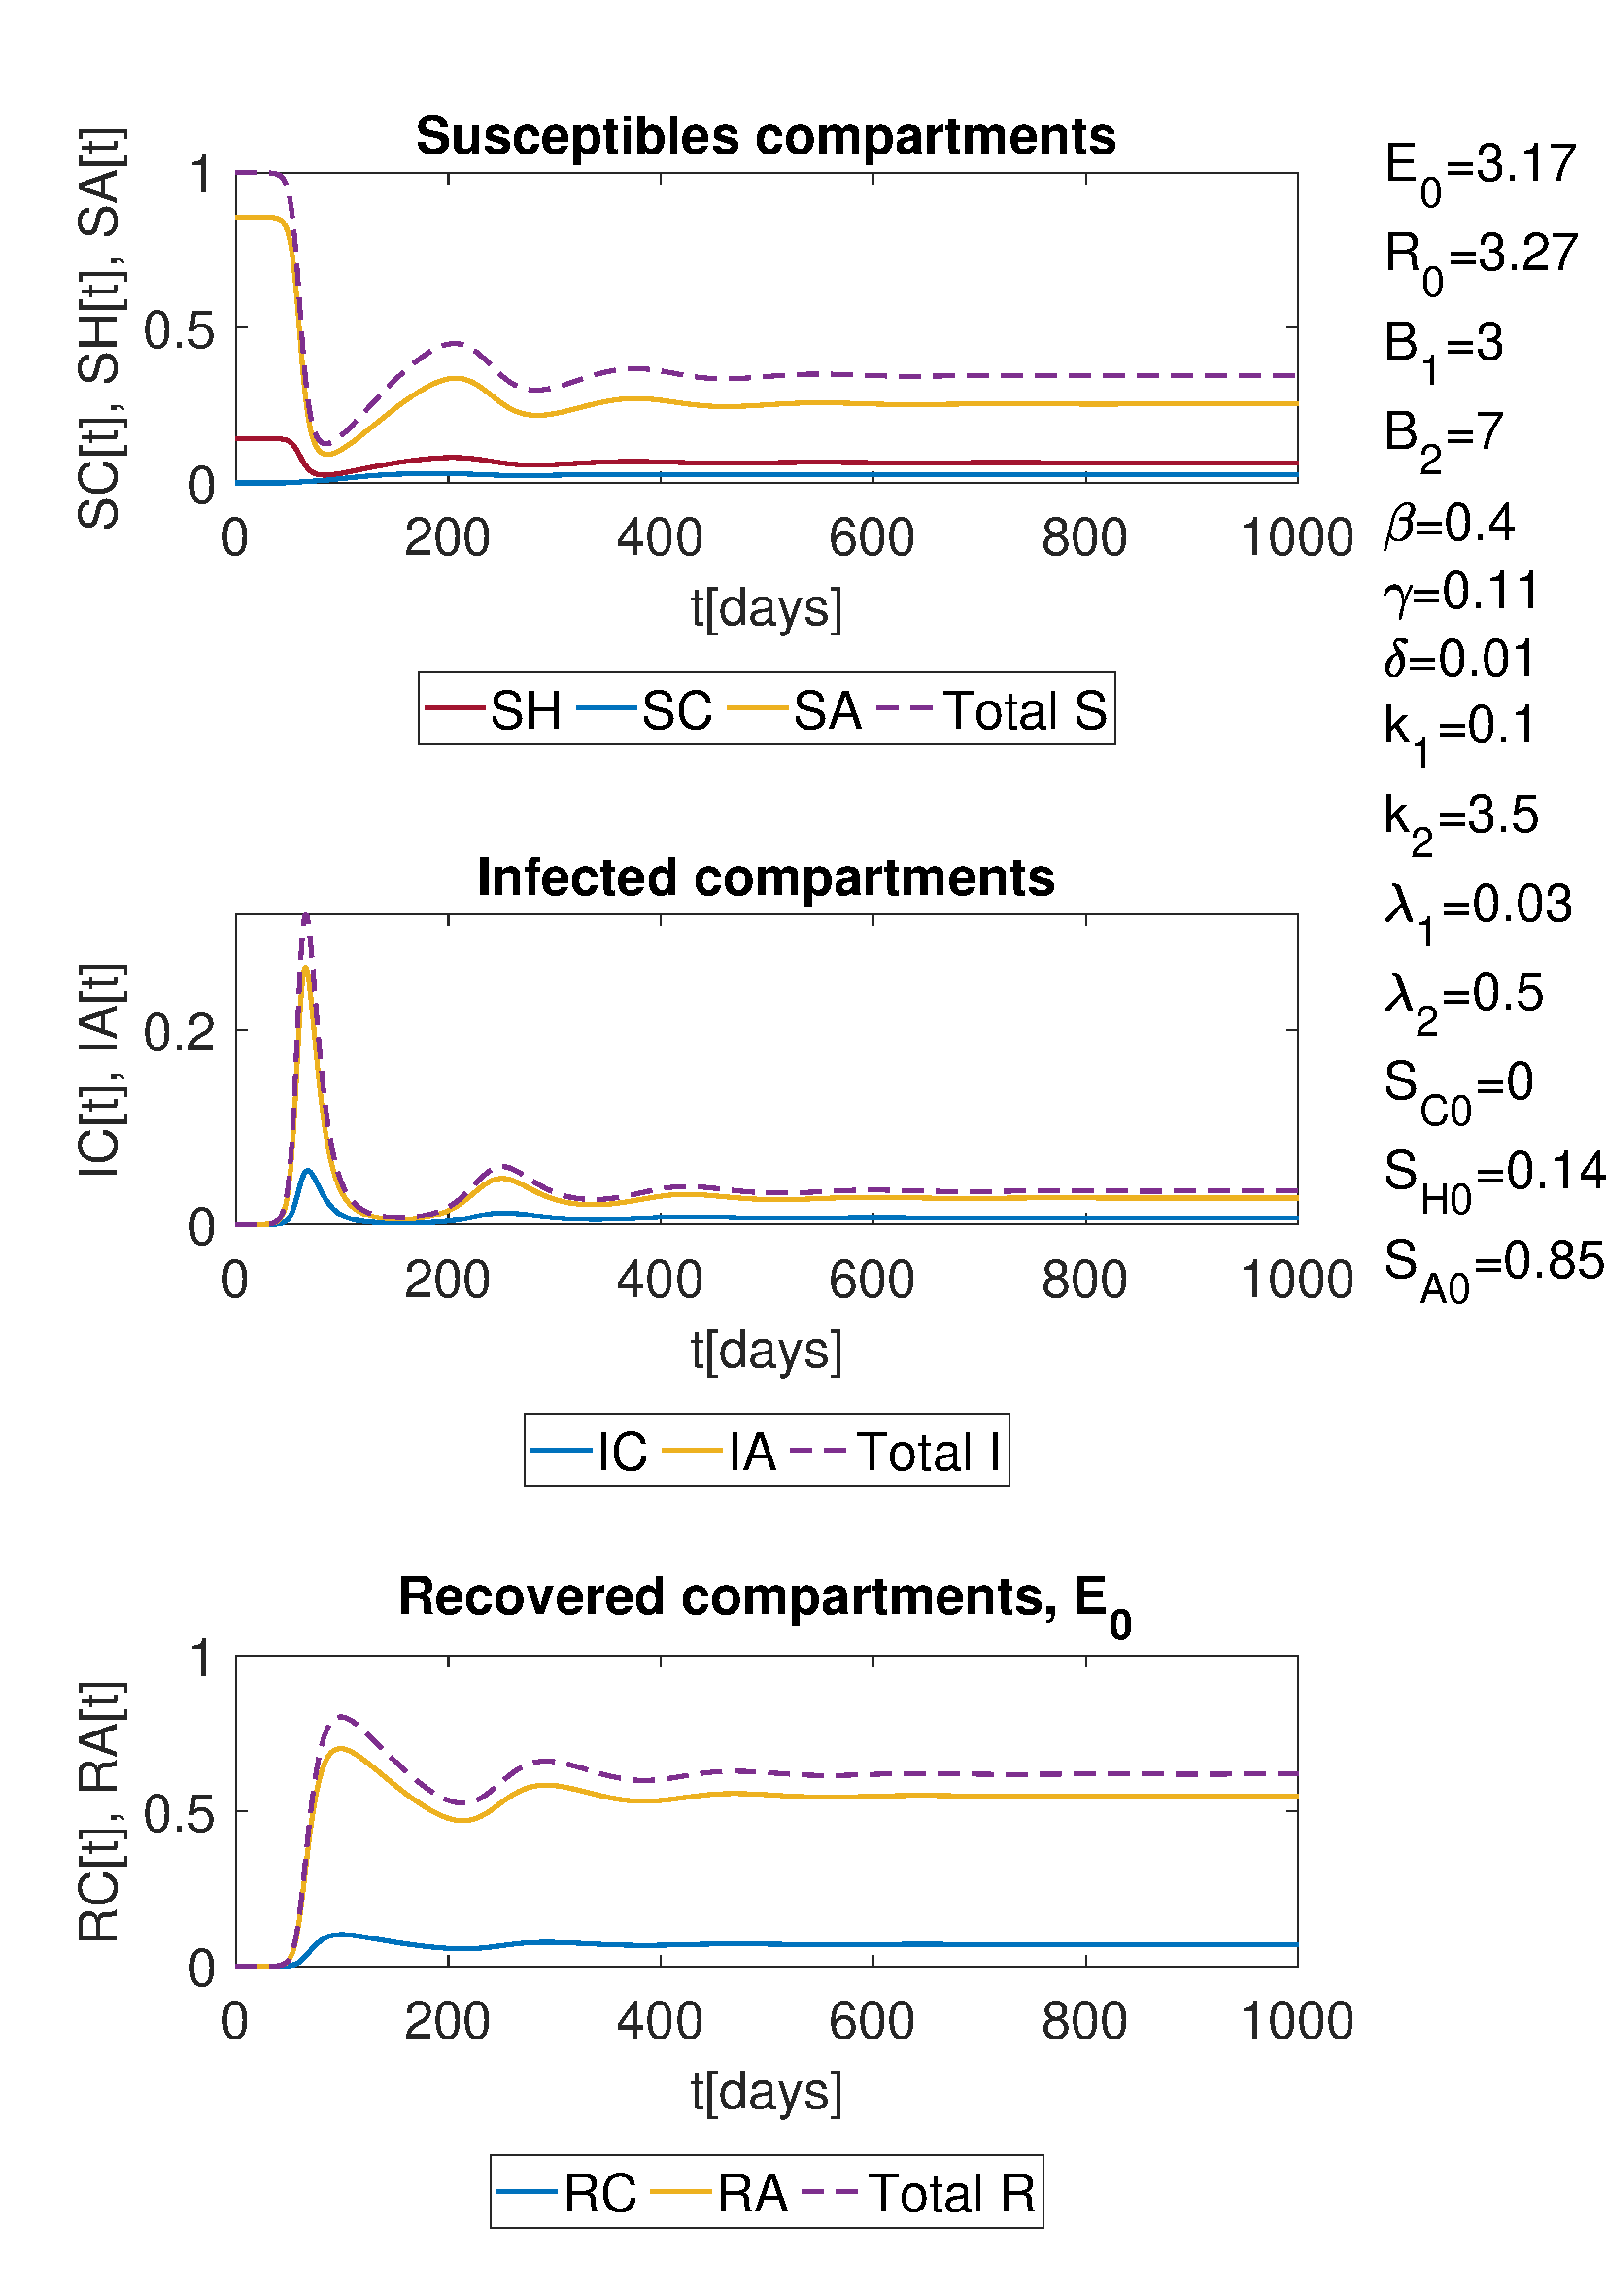
\includegraphics[width=0.5\linewidth]{1_corpo/figure/behav_epi_sim/E_0_model_3epi_behav_sim_B2_mag_B1}} 
	\caption[Full model simulation figure third]{V case.}
	\label{fig:sim_B1_less_B2}
\end{figure}

\subsection{Influence of the $\psi$ parameter}
To model how government policies can influence the behavior of the population and create a distinction between spontaneous behavior and reactions to regulations, the parameter $\psi$ was introduced. It acts as a central mean-field intervention, multiplying the coefficients $k_1$, $k_3$, and $k_5$.

The value of $\psi$ is greater than one ($\psi > 1$) when the simulations consider enforced policies that individuals must follow, and equal to one ($\psi = 1$) when no such regulations are in place.

In Figure \ref{fig:sim_psi}, the evolution of $S_C$ and the total number of infected individuals as $\psi$ varies is represented. It is evident that increasing the value of $\psi$ changes the timescale of compliance, causing $S_C$ to reach its maximum more quickly, while also increasing the final number of $S_C$. Furthermore, it significantly reduces the peak value of infected individuals.

This effect is very pronounced when comparing cases: with $\psi = 1$, the peak value of $I$ is around $2\%$, whereas in other cases, it drops to approximately $0.0007\%$.
\begin{figure}[ht]
	\centering
	\subfloat[][$S_C$ for varying $\psi$.]
	{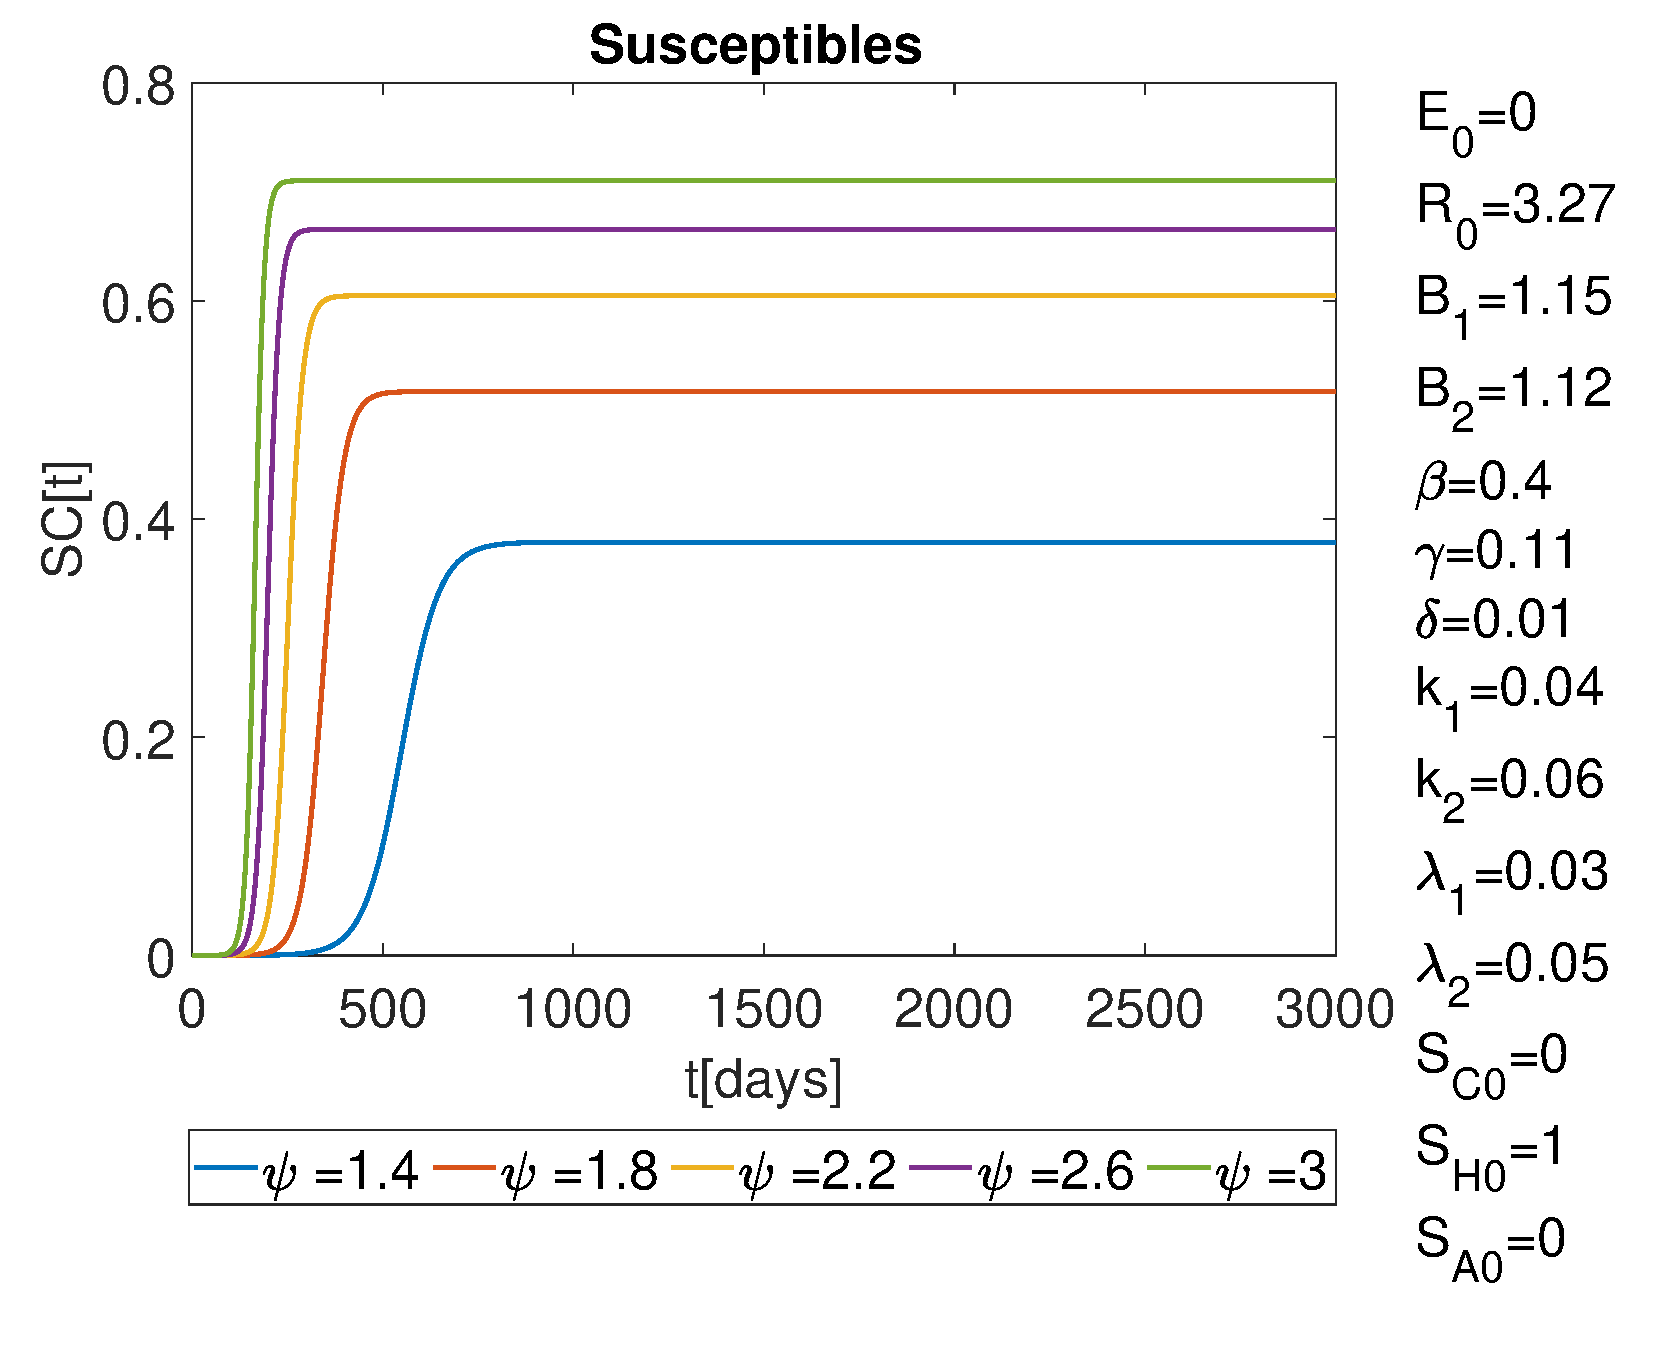
\includegraphics[width=0.6\linewidth]{1_corpo/figure/behav_epi_sim/E_0_model_1epi_behav_sim_psi}} \\
	\subfloat[][$I_{tot}$ for varying $\psi$.]
	{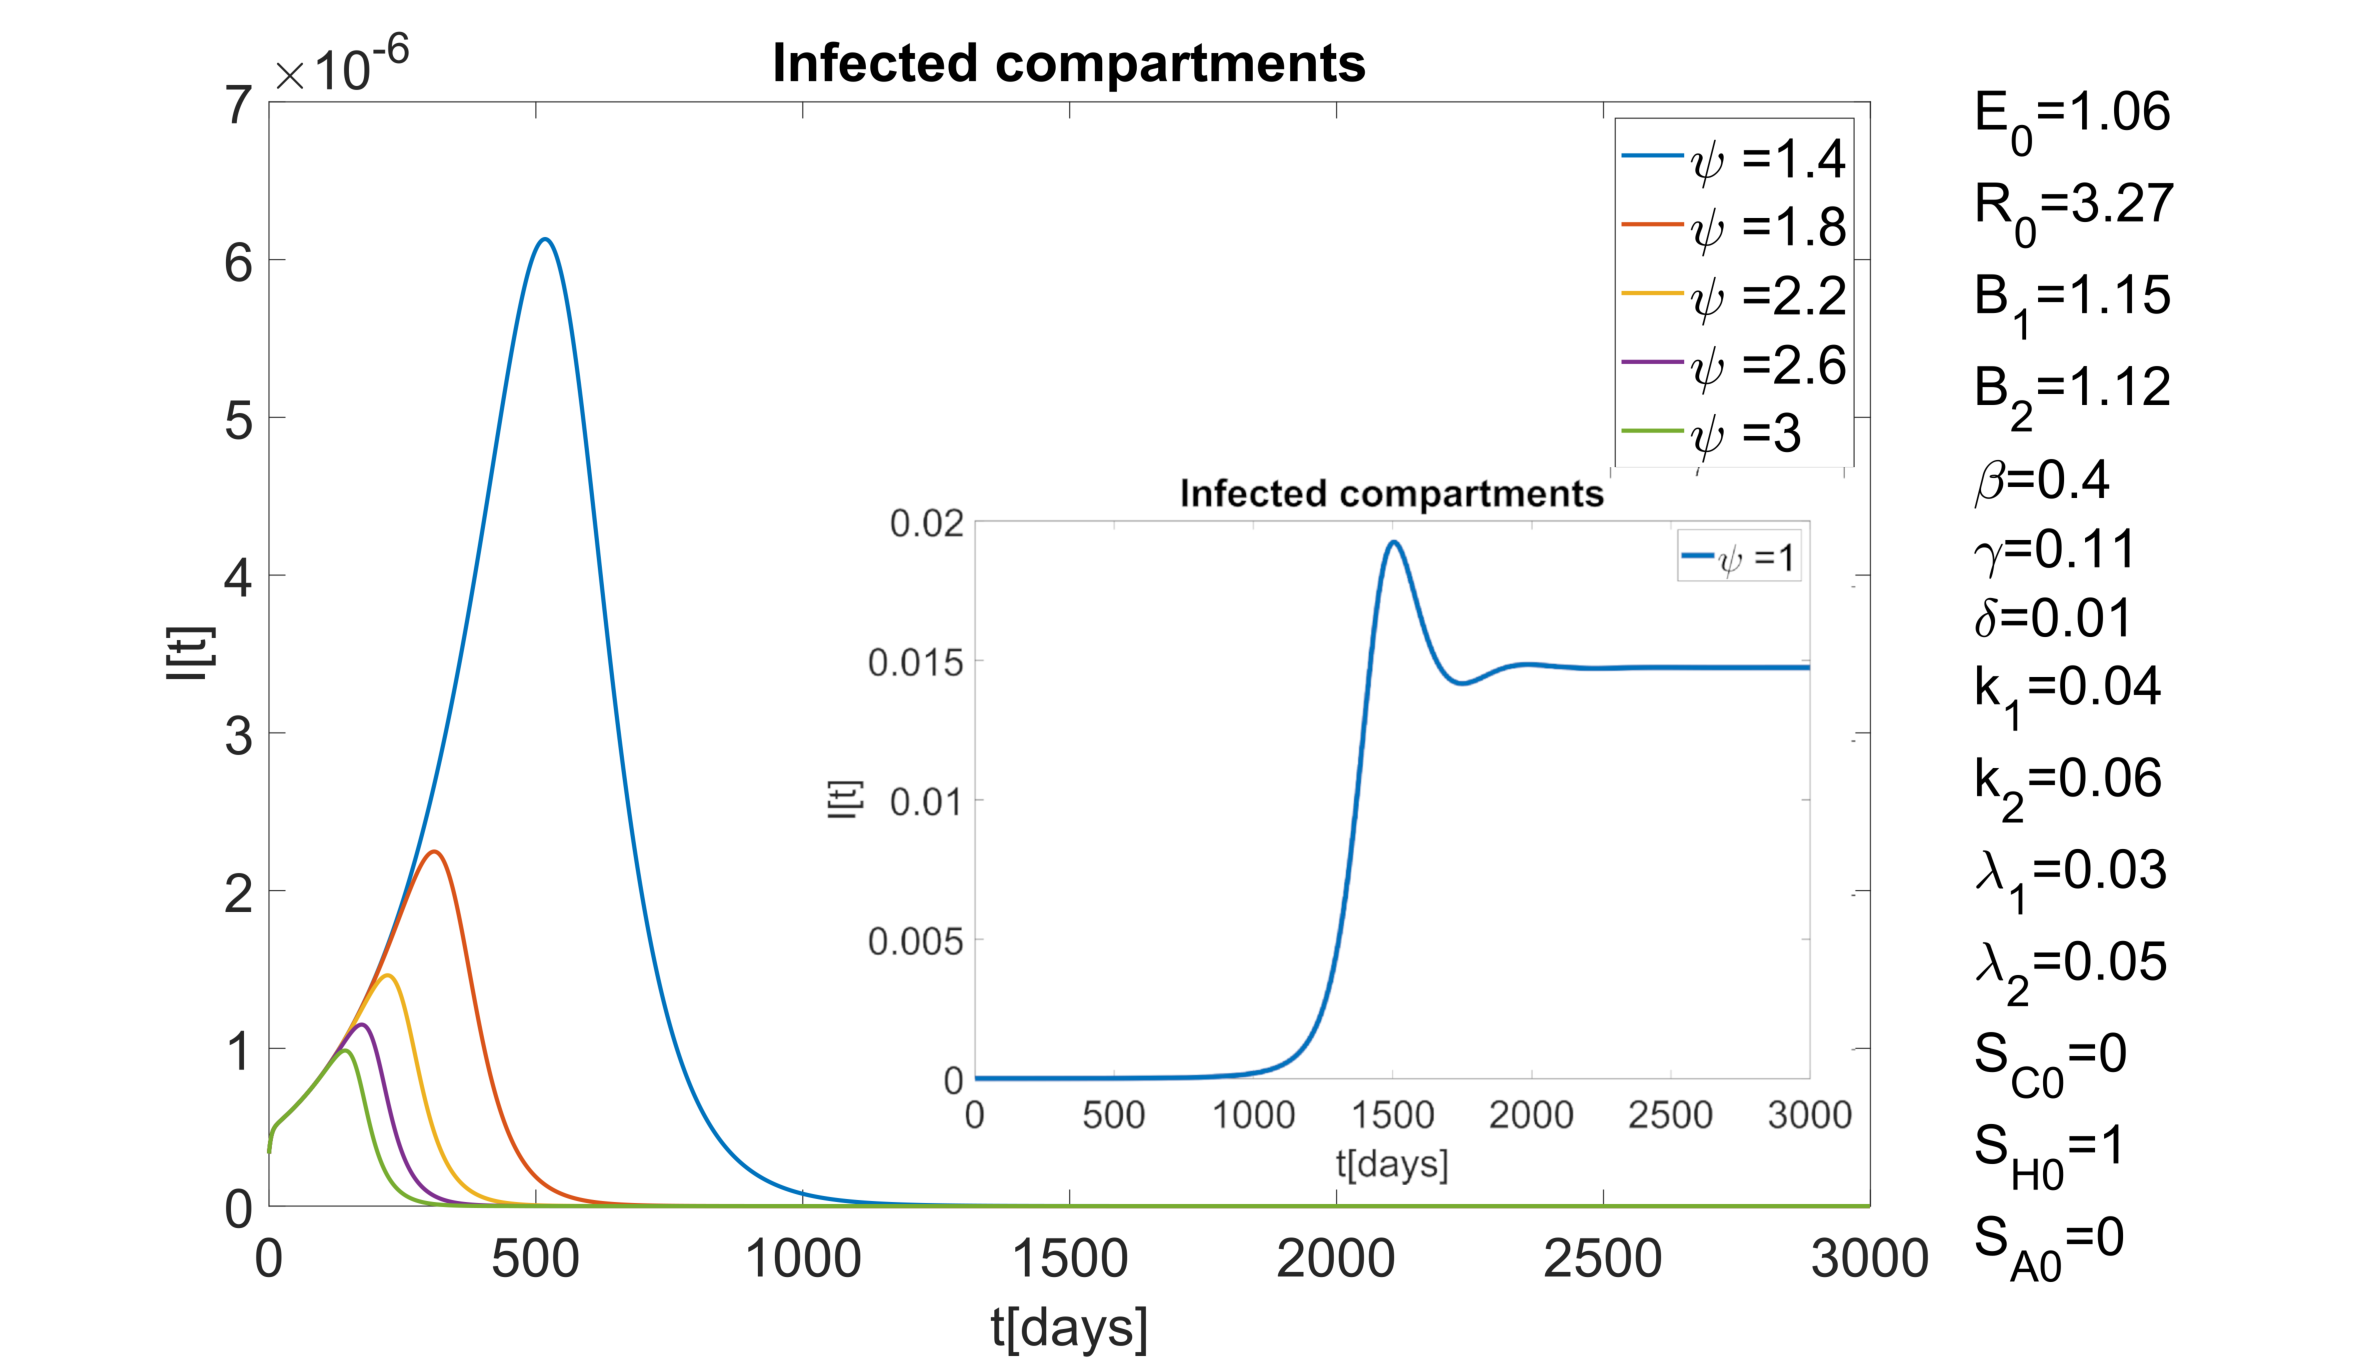
\includegraphics[width=0.68\linewidth]{1_corpo/figure/behav_epi_sim/E_0_model_3epi_behav_sim_psi}} \\
	\caption[Simulation varying $\psi$]{Simulations of the epidemic-behavioral model with varying parameter $\psi$. In the first figure, the changes in the $S_C$ curve are shown. The maximum is reached more quickly when $\psi > 1$. In the second figure, the corresponding $I = I_C + I_A$ curves are presented. The small panel represents the case with $\psi = 1$. For $\psi > 1$, the infection peak becomes significantly smaller.}
	\label{fig:sim_psi}
\end{figure}
\\
\\
Overall, the implemented multi-system model demonstrates its ability to adapt effectively to a variety of scenarios. Specifically, it captures both situations: one where Compliant behavior significantly mitigates the disease's impact, and the opposite scenario, where the dominant presence of the Against group triggers a disease outbreak. These outcomes arise under the same disease parameter values, $\beta, \gamma, \delta$. The estimated value of $E_0$ proves to be a valuable indicator of the stability of the system DFE. 
